%\subsubsection*{Transient}

\begin{figure}[ht!]
\centering\leavevmode
\begin{minipage}{17cm}
\centering\leavevmode
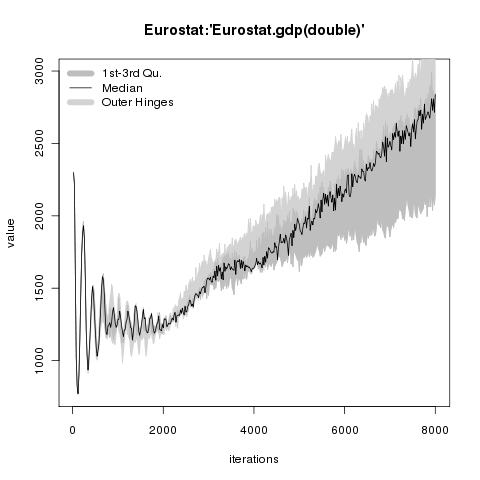
\includegraphics[width=8cm]{./transient/tax_0.05/Eurostat-gdp.png}
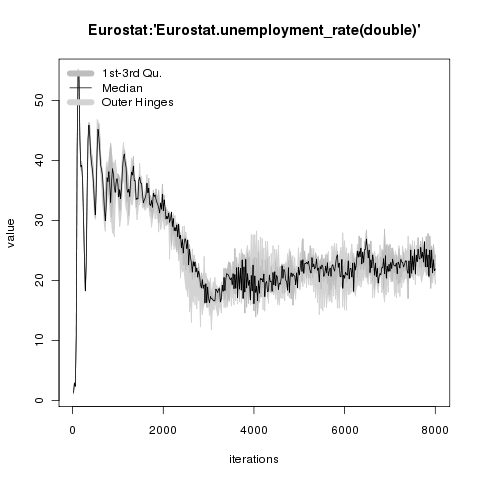
\includegraphics[width=8cm]{./transient/tax_0.05/Eurostat-unemployment_rate.png}\\
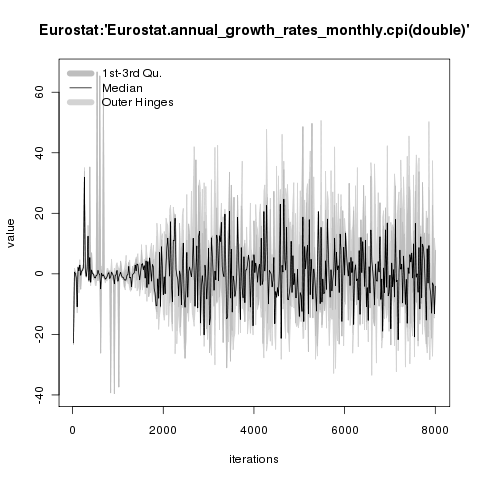
\includegraphics[width=8cm]{./transient/tax_0.05/Eurostat-cpi.png}
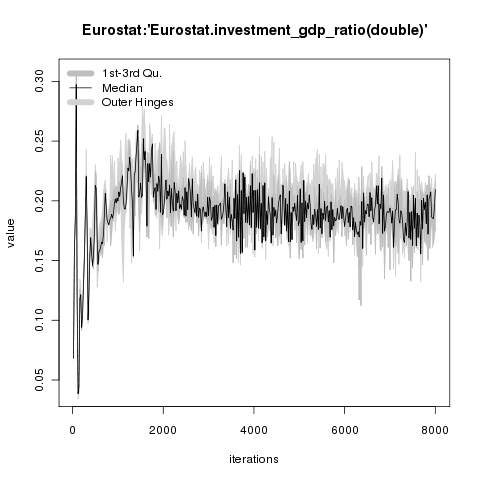
\includegraphics[width=8cm]{./transient/tax_0.05/Eurostat-investment_gdp_ratio.png}
\end{minipage}
\caption{Time series plots for 20 batch runs. GDP, unemployment rate, inflation rate and investment/GDP ratio. Data: $4000-8000$.}
\label{Figure: transient time}
\end{figure}

%\subsubsection*{Distribution across batch runs}

\begin{figure}[ht!]
\centering\leavevmode
\begin{minipage}{17cm}
\centering\leavevmode
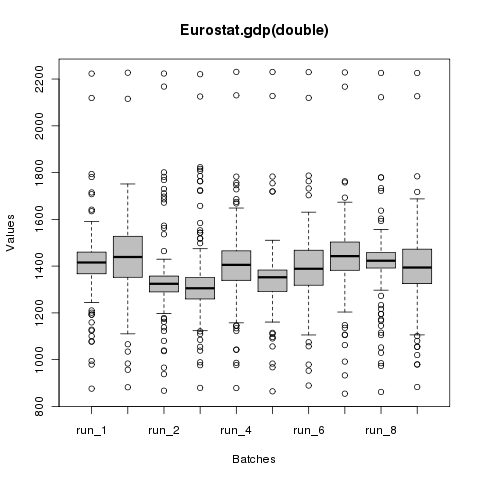
\includegraphics[width=8cm]{./batch/tax_0.05/Eurostat-gdp-runbatch.png}
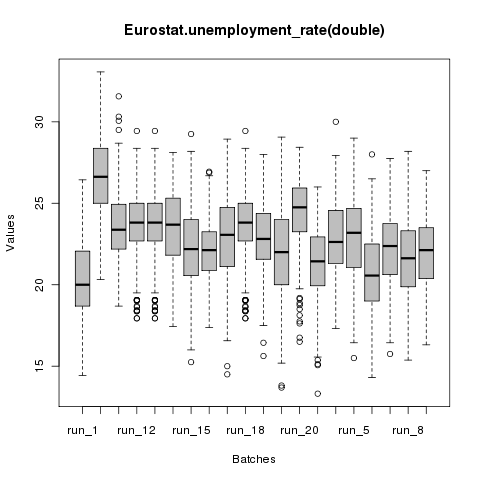
\includegraphics[width=8cm]{./batch/tax_0.05/Eurostat-unemployment_rate-runbatch.png}\\
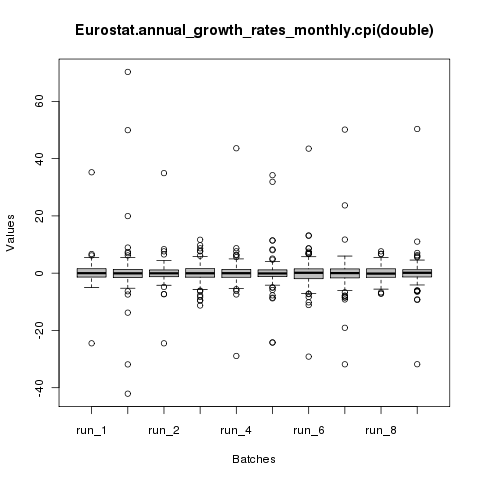
\includegraphics[width=8cm]{./batch/tax_0.05/Eurostat-cpi-runbatch.png}
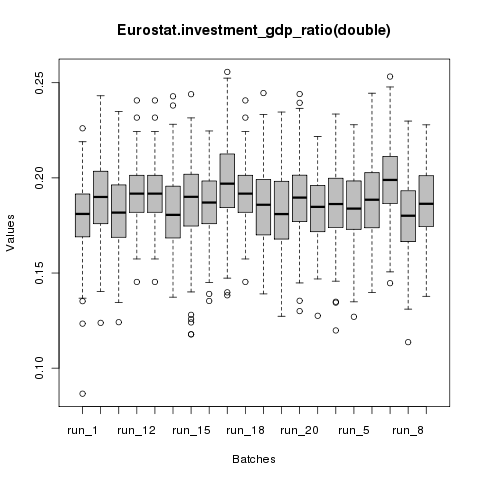
\includegraphics[width=8cm]{./batch/tax_0.05/Eurostat-investment_gdp_ratio-runbatch.png}
\end{minipage}
\caption{Box plots for separate runs of GDP, unemployment rate, inflation rate and investment/GDP ratio. Data: $4000-8000$.}
\label{Figure: run batch}
\end{figure}
